% Исследовательская часть
\section{Исследовательская часть}

\subsection{Пример работы программы}

\hspace{1.25cm}
Работа разработанной программы на тестовых входных данных для решения задачи коммивояжёра полным перебором и муравьиным алгоритмом приведена на рисунке~\ref{fig:example}.

\begin{figure}[H]
    \centering
    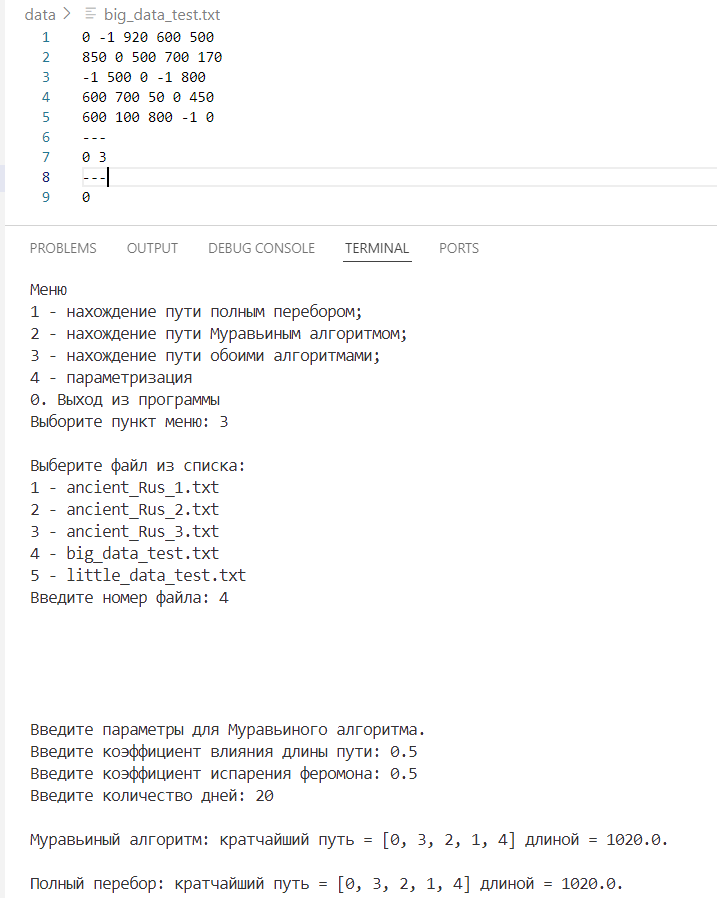
\includegraphics[width=1\textwidth]{img/example.png}
    \caption{Пример работы программы.}
    \label{fig:example} % Метка для ссылки на картинку
\end{figure}


\subsection{Результаты параметризации}

\hspace{1.25cm}
Для определения комбинации параметров муравьиного алгоритма, которые позволяют получать ответ, наиболее близкий к результату полного перебора для выбранного класса данных была выполнена автоматическая параметризация на трёх классах данных. Для каждого класса была составлена таблица с входными параметрами и получившимися результатами, которая включает в себя следующие колонки:

\begin{enumerate}[label=\arabic*)]
    \item $\alpha$ -- параметр влияния длины пути;
    \item $\beta$ -- параметр влияния феромона;
    \item $\rho$ -- коэффициент испарения феромона;
    \item дни -- количество дней жизни колонии муравьёв;
    \item результат АПП -- результат, полученный алгоритмом полного перебора;
    \item результат МА -- результат, полученный муравьиным алгоритмом на данных параметрах;
    \item разница -- разность результата МА с результатом АПП.
\end{enumerate}

\subsubsection{Класс данных №1}

\hspace{1.25cm}
Класс данных №1 собой представляет собой матрицу смежности размером $10 \times 10$, элементы которой являются расстояниями между городами России, 3 реки, сезон зимний. Таблица~\ref{tab:class_1} содержит параметры и результаты для первого класса данных.

Матрица смежностей для класса данных №1:

\begin{equation*}
\begin{bmatrix}
0  &  450 & 700 & -1 &  320 & 500 & 650 & -1 &  400 & 580 \\
450 & 0  &  350 & -1 &  -1 &  -1 &  300 & 700 & -1 &  450 \\
700 & 350 & 0  &  200 & 500 & -1 &  450 & -1 &  -1 &  600 \\
-1 &  -1 &  200 & 0  &  400 & 550 & -1 &  300 & 650 & -1 \\
320 & -1 &  500 & 400 & 0  &  -1 &  -1  & -1 &  300 & 100 \\
500 & -1 &  -1 &  550 & -1 &  0  &  -1  & 400 & -1 &  -1 \\
650 & 300 & 450 & -1  & -1  & -1 &  0  &  350 & -1  & 200 \\
-1 &  700 & -1 &  300 & -1 &  400 & 350 & 0  &  550 & -1 \\
400 & -1  & -1  & 650 & 300 & -1 &  -1 &  550 & 0  &  250 \\
580 & 450 & 600 & -1 &  100 & -1 &  200 & -1 &  250 & 0 \\
\end{bmatrix}
\end{equation*}
Направления рек: $(2 \to 3)$, $(5 \to 8)$ и $(7 \to 1)$.

\begin{table}[H]
    \centering
    \caption{Параметры для класса данных №1}
    \label{tab:class_1}
    \begin{tabular}{|c|c|c|c|c|c|c|}
        \hline
        $\alpha$ & $\beta$ & $\rho$ & дни & результат АПП & результат МА & разница \\
        \hline
  0.10 &   0.90 &   0.10 &      1 &    2550.00 &    2900.00 &     350.00  \\
  0.10 &   0.90 &   0.10 &      3 &    2550.00 &    3000.00 &     450.00  \\
  0.10 &   0.90 &   0.10 &      5 &    2550.00 &    2720.00 &     170.00  \\
  0.10 &   0.90 &   0.10 &     10 &    2550.00 &    2770.00 &     220.00  \\
  0.10 &   0.90 &   0.10 &     30 &    2550.00 &    2570.00 &      20.00  \\
  0.10 &   0.90 &   0.10 &     60 &    2550.00 &    2550.00 &       0.00  \\
  0.10 &   0.90 &   0.10 &    100 &    2550.00 &    2580.00 &      30.00  \\
  0.10 &   0.90 &   0.10 &    150 &    2550.00 &    2580.00 &      30.00  \\
  0.10 &   0.90 &   0.10 &    200 &    2550.00 &    2550.00 &       0.00  \\
  0.10 &   0.90 &   0.10 &    300 &    2550.00 &    2630.00 &      80.00  \\
  0.10 &   0.90 &   0.20 &      1 &    2550.00 &    3570.00 &    1020.00  \\
  0.10 &   0.90 &   0.20 &      3 &    2550.00 &    3150.00 &     600.00  \\
  0.10 &   0.90 &   0.20 &      5 &    2550.00 &    2900.00 &     350.00  \\
  0.10 &   0.90 &   0.20 &     10 &    2550.00 &    2750.00 &     200.00  \\
  0.10 &   0.90 &   0.20 &     30 &    2550.00 &    2750.00 &     200.00  \\
  ... &   ... &   ... &    ... &    ... &    ... &      ...  \\
   0.60 &   0.40 &   0.40 &      1 &    2550.00 &    3350.00 &     800.00  \\
  0.60 &   0.40 &   0.40 &      3 &    2550.00 &    3070.00 &     520.00  \\
  0.60 &   0.40 &   0.40 &      5 &    2550.00 &    3150.00 &     600.00  \\
  0.60 &   0.40 &   0.40 &     10 &    2550.00 &    2870.00 &     320.00  \\
  0.60 &   0.40 &   0.40 &     30 &    2550.00 &    2850.00 &     300.00  \\
  0.60 &   0.40 &   0.40 &     60 &    2550.00 &    2650.00 &     100.00  \\
  0.60 &   0.40 &   0.40 &    100 &    2550.00 &    2650.00 &     100.00  \\
  0.60 &   0.40 &   0.40 &    150 &    2550.00 &    2600.00 &      50.00  \\
  0.60 &   0.40 &   0.40 &    200 &    2550.00 &    2620.00 &      70.00  \\
  0.60 &   0.40 &   0.40 &    300 &    2550.00 &    2550.00 &       0.00  \\
    ... &   ... &   ... &    ... &    ... &    ... &      ...  \\
      0.90 &   0.10 &   0.80 &    300 &    2550.00 &    2650.00 &     100.00  \\
  0.90 &   0.10 &   0.90 &      1 &    2550.00 &    3520.00 &     970.00  \\
  0.90 &   0.10 &   0.90 &      3 &    2550.00 &    3170.00 &     620.00  \\
  0.90 &   0.10 &   0.90 &      5 &    2550.00 &    3080.00 &     530.00  \\
  0.90 &   0.10 &   0.90 &     10 &    2550.00 &    2970.00 &     420.00  \\
  0.90 &   0.10 &   0.90 &     30 &    2550.00 &    2900.00 &     350.00  \\
  0.90 &   0.10 &   0.90 &     60 &    2550.00 &    2750.00 &     200.00  \\
  0.90 &   0.10 &   0.90 &    100 &    2550.00 &    2800.00 &     250.00  \\
  0.90 &   0.10 &   0.90 &    150 &    2550.00 &    2600.00 &      50.00  \\
  0.90 &   0.10 &   0.90 &    200 &    2550.00 &    2650.00 &     100.00  \\
  0.90 &   0.10 &   0.90 &    300 &    2550.00 &    2620.00 &      70.00  \\
  \hline
    \end{tabular}
\end{table}

Наилучшими параметрами по результатам данного измерения для класса №1 были выбраны   $\alpha$ = 0.50, $\beta$ = 0.50, $\rho$ = 0.90 и количество дней $\geq$ 100.

\subsubsection{Класс данных №2}

\hspace{1.25cm}
Класс данных №2 собой представляет собой матрицу смежности размером $10 \times 10$, элементы которой являются расстояниями между городами России, 2 реки, сезон летний. Таблица~\ref{tab:class_2} содержит параметры и результаты для второго класса данных.

Матрица смежностей для класса данных №2:

\begin{equation*}
\begin{bmatrix}
0  &  300 & -1 &  450 & 600 & -1 &  500 & 700 & -1 &  -1 \\
300 & 0  &  350 & -1  & -1 &  200 & -1 &  -1  & 650 & -1 \\
-1 &  350 & 0  &  200 & -1 &  -1  & -1 &  400 & -1  & 300 \\
450 & -1 &  200 & 0  &  -1 &  550 & -1  & -1  & 600 & -1 \\
600 & -1 &  -1 &  -1 &  0  &  -1 &  300 & 700 & -1  & -1 \\
-1 &  200 & -1 &  550 & -1 &  0  &  400 & -1  & -1  & -1 \\
500 & -1  & -1 &  -1 &  300 & 400 & 0  &  -1  & 250 & -1 \\
700 & -1 &  400 & -1 &  700 & -1 &  -1 &  0  &  -1 &  450 \\
-1 &  650 & -1 &  600 & -1 &  -1 &  250 & -1 &  0  &  200 \\
-1 &  -1 &  300 & -1 &  -1  & -1 &  -1  & 450 & 200 & 0 \\
\end{bmatrix}
\end{equation*}
Направления рек: $(4 \to 6)$ и $(9 \to 7)$.

\begin{table}[H]
    \centering
    \caption{Параметры для класса данных №2}
    \label{tab:class_2}
    \begin{tabular}{|c|c|c|c|c|c|c|}
        \hline
        $\alpha$ & $\beta$ & $\rho$ & дни & результат АПП & результат МА & разница \\
        \hline
  0.10 &   0.90 &   0.10 &      1 &    2375.00 &    2475.00 &     100.00  \\
  0.10 &   0.90 &   0.10 &      3 &    2375.00 &    3075.00 &     700.00  \\
  0.10 &   0.90 &   0.10 &      5 &    2375.00 &    2825.00 &     450.00  \\
  0.10 &   0.90 &   0.10 &     10 &    2375.00 &    2525.00 &     150.00  \\
  0.10 &   0.90 &   0.10 &     30 &    2375.00 &    2475.00 &     100.00  \\
  0.10 &   0.90 &   0.10 &     60 &    2375.00 &    2475.00 &     100.00  \\
  0.10 &   0.90 &   0.10 &    100 &    2375.00 &    2375.00 &       0.00  \\
  0.10 &   0.90 &   0.10 &    150 &    2375.00 &    2375.00 &       0.00  \\
  0.10 &   0.90 &   0.10 &    200 &    2375.00 &    2375.00 &       0.00  \\
  0.10 &   0.90 &   0.10 &    300 &    2375.00 &    2375.00 &       0.00  \\
  0.10 &   0.90 &   0.20 &      1 &    2375.00 &    3475.00 &    1100.00  \\
  0.10 &   0.90 &   0.20 &      3 &    2375.00 &    2925.00 &     550.00  \\
  0.10 &   0.90 &   0.20 &      5 &    2375.00 &    2775.00 &     400.00  \\
  0.10 &   0.90 &   0.20 &     10 &    2375.00 &    2850.00 &     475.00  \\
  0.10 &   0.90 &   0.20 &     30 &    2375.00 &    2375.00 &       0.00  \\
  0.10 &   0.90 &   0.20 &     60 &    2375.00 &    2375.00 &       0.00  \\
  ... &   ... &   ... &    ... &    ... &    ... &      ...  \\
  0.60 &   0.40 &   0.40 &      1 &    2375.00 &    2625.00 &     250.00  \\
  0.60 &   0.40 &   0.40 &      3 &    2375.00 &    2875.00 &     500.00  \\
  0.60 &   0.40 &   0.40 &      5 &    2375.00 &    2775.00 &     400.00  \\
  0.60 &   0.40 &   0.40 &     10 &    2375.00 &    2525.00 &     150.00  \\
  0.60 &   0.40 &   0.40 &     30 &    2375.00 &    2775.00 &     400.00  \\
  0.60 &   0.40 &   0.40 &     60 &    2375.00 &    2375.00 &       0.00  \\
  0.60 &   0.40 &   0.40 &    100 &    2375.00 &    2675.00 &     300.00  \\
  0.60 &   0.40 &   0.40 &    150 &    2375.00 &    2475.00 &     100.00  \\
  0.60 &   0.40 &   0.40 &    200 &    2375.00 &    2375.00 &       0.00  \\
  0.60 &   0.40 &   0.40 &    300 &    2375.00 &    2375.00 &       0.00  \\
    ... &   ... &   ... &    ... &    ... &    ... &      ...  \\
  0.90 &   0.10 &   0.90 &      3 &    2375.00 &    3275.00 &     900.00  \\
  0.90 &   0.10 &   0.90 &      5 &    2375.00 &    2525.00 &     150.00  \\
  0.90 &   0.10 &   0.90 &     10 &    2375.00 &    2525.00 &     150.00  \\
  0.90 &   0.10 &   0.90 &     30 &    2375.00 &    2775.00 &     400.00  \\
  0.90 &   0.10 &   0.90 &     60 &    2375.00 &    2375.00 &       0.00  \\
  0.90 &   0.10 &   0.90 &    100 &    2375.00 &    2475.00 &     100.00  \\
  0.90 &   0.10 &   0.90 &    150 &    2375.00 &    2725.00 &     350.00  \\
  0.90 &   0.10 &   0.90 &    200 &    2375.00 &    2375.00 &       0.00  \\
  0.90 &   0.10 &   0.90 &    300 &    2375.00 &    2475.00 &     100.00  \\
  \hline
    \end{tabular}
\end{table}

Наилучшими параметрами по результатам данного измерения для класса №2 были выбраны   $\alpha$ = 0.30, $\beta$ = 0.70, $\rho$ = 0.30 и количество дней $\geq$ 30.


\subsubsection{Класс данных №3}

\hspace{1.25cm}
Класс данных №3 собой представляет собой матрицу смежности размером $10 \times 10$, элементы которой являются расстояниями между городами России, 2 реки, сезон летний, в графе малое количество рёбер. Таблица~\ref{tab:class_3} содержит параметры и результаты для третьего класса данных.

Матрица смежностей для класса данных №3:

\begin{equation*}
\begin{bmatrix}
0   & -1 &  300 & 450 & -1 &  200 & -1  & -1  & -1 &  100 \\
-1 &  0 &   400 & -1 &  600 & -1 &  500 & -1 &  -1  & -1 \\
300 & 400 & 0   & -1 &  -1 &  -1 &  -1 &  -1  & -1  & -1 \\
450 & -1 &  -1 &  0  &  -1 &  700 & 200 & -1 &  650 & -1 \\
-1  & 600 & -1 &  -1 &  0 &   400 & -1  & -1 &  -1  & -1 \\
200 & -1 &  -1  & 700 & 400 & 0  &  -1 &  300 & -1  & 450 \\
-1  & 500 & -1 &  200 & -1 &  -1 &  0  &  -1 &  600 & -1 \\
-1  & -1  & -1 &  -1 &  -1 &  300 & -1  & 0  &  500 & -1 \\
-1  & -1 &  -1 &  650 & -1  & -1 &  600 & 500 & 0  &  -1 \\
100 & -1  & -1 &  -1 &  -1 &  450 & -1 &  -1 &  -1 &  0 \\
\end{bmatrix}
\end{equation*}
Направления рек: $(1 \to 5)$ и $(6 \to 10)$.

\begin{table}[H]
    \centering
    \caption{Параметры для класса данных №3}
    \label{tab:class_3}
    \begin{tabular}{|c|c|c|c|c|c|c|}
        \hline
        $\alpha$ & $\beta$ & $\rho$ & дни & результат АПП & результат МА & разница \\
        \hline
  0.10 &   0.90 &   0.10 &      1 &    3350.00 &    3450.00 &     100.00  \\
  0.10 &   0.90 &   0.10 &      3 &    3350.00 &    3500.00 &     150.00  \\
  0.10 &   0.90 &   0.10 &      5 &    3350.00 &    3350.00 &       0.00  \\
  0.10 &   0.90 &   0.10 &     10 &    3350.00 &    3400.00 &      50.00  \\
  0.10 &   0.90 &   0.10 &     30 &    3350.00 &    3350.00 &       0.00  \\
  0.10 &   0.90 &   0.10 &     60 &    3350.00 &    3350.00 &       0.00  \\
  0.10 &   0.90 &   0.10 &    100 &    3350.00 &    3350.00 &       0.00  \\
  0.10 &   0.90 &   0.10 &    150 &    3350.00 &    3350.00 &       0.00  \\
  0.10 &   0.90 &   0.10 &    200 &    3350.00 &    3350.00 &       0.00  \\
  0.10 &   0.90 &   0.10 &    300 &    3350.00 &    3350.00 &       0.00  \\
  0.10 &   0.90 &   0.20 &      1 &    3350.00 &    3500.00 &     150.00  \\
  0.10 &   0.90 &   0.20 &      3 &    3350.00 &    3350.00 &       0.00  \\
  0.10 &   0.90 &   0.20 &      5 &    3350.00 &    3450.00 &     100.00  \\
  0.10 &   0.90 &   0.20 &     10 &    3350.00 &    3400.00 &      50.00  \\
  0.10 &   0.90 &   0.20 &     30 &    3350.00 &    3350.00 &       0.00  \\
  0.10 &   0.90 &   0.20 &     60 &    3350.00 &    3350.00 &       0.00  \\
  0.10 &   0.90 &   0.20 &    100 &    3350.00 &    3350.00 &       0.00  \\
  0.10 &   0.90 &   0.20 &    150 &    3350.00 &    3350.00 &       0.00  \\
  0.10 &   0.90 &   0.20 &    200 &    3350.00 &    3350.00 &       0.00  \\
  0.10 &   0.90 &   0.20 &    300 &    3350.00 &    3350.00 &       0.00  \\
  ... &   ... &   ... &    ... &    ... &    ... &      ...  \\
  0.50 &   0.50 &   0.80 &    300 &    3350.00 &    3350.00 &       0.00  \\
  0.50 &   0.50 &   0.90 &      1 &    3350.00 &    3800.00 &     450.00  \\
  0.50 &   0.50 &   0.90 &      3 &    3350.00 &    3350.00 &       0.00  \\
  0.50 &   0.50 &   0.90 &      5 &    3350.00 &    3350.00 &       0.00  \\
  0.50 &   0.50 &   0.90 &     10 &    3350.00 &    3350.00 &       0.00  \\
  0.50 &   0.50 &   0.90 &     30 &    3350.00 &    3350.00 &       0.00  \\
  0.50 &   0.50 &   0.90 &     60 &    3350.00 &    3350.00 &       0.00  \\
  0.50 &   0.50 &   0.90 &    100 &    3350.00 &    3350.00 &       0.00  \\
  0.50 &   0.50 &   0.90 &    150 &    3350.00 &    3350.00 &       0.00  \\
  0.50 &   0.50 &   0.90 &    200 &    3350.00 &    3350.00 &       0.00  \\
  0.50 &   0.50 &   0.90 &    300 &    3350.00 &    3350.00 &       0.00  \\
    ... &   ... &   ... &    ... &    ... &    ... &      ...  \\
  0.90 &   0.10 &   0.90 &      5 &    3350.00 &    3350.00 &       0.00  \\
  0.90 &   0.10 &   0.90 &     10 &    3350.00 &    3450.00 &     100.00  \\
  0.90 &   0.10 &   0.90 &     30 &    3350.00 &    3350.00 &       0.00  \\
  0.90 &   0.10 &   0.90 &     60 &    3350.00 &    3350.00 &       0.00  \\
  0.90 &   0.10 &   0.90 &    100 &    3350.00 &    3350.00 &       0.00  \\
  0.90 &   0.10 &   0.90 &    150 &    3350.00 &    3350.00 &       0.00  \\
  0.90 &   0.10 &   0.90 &    200 &    3350.00 &    3350.00 &       0.00  \\
  0.90 &   0.10 &   0.90 &    300 &    3350.00 &    3350.00 &       0.00  \\
  \hline
    \end{tabular}
\end{table}

В связи с малым количеством рёбер муравьиный алгоритм практически на всех параметрах выдаёт значения идентичные или близкие к результатам полного перебора. Особо лишь хочется отметить, что расхождения в основном наблюдаются при количество дней меньше 10.


\subsubsection*{Выводы}

\hspace{1.25cm}
В данном разделе был приведён пример работы программы, а также проведена автоматическая параметризация для определения наилучших параметров для муравьиного алгоритма на трёх различных входных данных. Была замечена зависимость точности муравьиного алгоритма в зависимости от количества рёбер в графе и числа дней жизни муравьиной колонии. 

\newpage